\documentclass[11pt, oneside]{article}   	% use "amsart" instead of "article" for AMSLaTeX format
\usepackage{geometry}                		% See geometry.pdf to learn the layout options. There are lots.
\geometry{letterpaper}                   		% ... or a4paper or a5paper or ... 
%\geometry{landscape}                		% Activate for rotated page geometry
%\usepackage[parfill]{parskip}    		% Activate to begin paragraphs with an empty line rather than an indent
\usepackage{graphicx}				% Use pdf, png, jpg, or eps§ with pdflatex; use eps in DVI mode
								% TeX will automatically convert eps --> pdf in pdflatex		
\usepackage{amsmath}
\usepackage{amssymb}
\usepackage{float}
\usepackage{hyperref}
\usepackage{wrapfig}
\usepackage{refcount}
\usepackage{gensymb}
\usepackage{tikz}
\usetikzlibrary{positioning}

\hypersetup{
    colorlinks=true,
    linkcolor=black,   
    urlcolor=cyan,
}

\newtheorem{innercustomthm}{Answer}
\newenvironment{answer}[1]
  {\renewcommand\theinnercustomthm{#1}\innercustomthm}
  {\endinnercustomthm}

\newtheorem{thm}{Theorem}
\newtheorem{conj}{Conjecture}
\newtheorem{question}{Question}
\newtheorem{idea}{Idea}
\newtheorem{postidea}{Post Idea}
\newtheorem{defn}{Definition}
\newtheorem{ans}{Answer}
\newtheorem{prop}{Property}
\newtheorem{propn}{Proposition}
\newtheorem{claim}{Claim}
\newtheorem{obs}{Observation}
\newtheorem{argt}{Argument}

\newcommand{\up}[1]{\ensuremath{^\text{#1}}}

\newcommand{\Q}{\mathbb{Q}}
\newcommand{\R}{\mathbb{R}}
\newcommand{\D}{\mathbb{D}}
\newcommand{\Z}{\mathbb{Z}}

\newcommand{\spacer}[1]{\rule[-#1]{0pt}{#1}}

\newcommand{\qed}{\ensuremath{\Box}}
\newcommand\bpf[1][]{\smallskip\noindent{\bf Proof#1.}\quad}
\newcommand\epf{\qed\medskip}
\newcommand\hr{\bigskip\hrule\bigskip}

\begin{document}

{\bf Truth Is Not the Bedrock of Human Knowledge}

Tyler Neylon

\bigskip

This article explores the question:
\begin{question}\label{q1}
    What is truth?
\end{question}

I'll tell you why this question is useful for any explorer of knowledge, and
I'll argue that our concept of truth is a human invention as opposed to an idea
that is intrinsic to the universe.
Moreover, the concept of truth has arbitrary aspects to it, meaning that some of
the things we consider to be true are less elegant and more anthropocentric than
we may first realize. This has profound ramifications on how we, humans, ought
to view both ourselves and the world.

\section{The Box We'll Peek Inside}

A lot of philosophy is poorly motivated, so I'll start by
looking at what useful results can come out of this exploration.

As a kid, I was taught {\em the scientific method} as a way to
learn about the world -- to learn what is true.
I'll roughly summarize the scientific method as the statement
of a hypothesis, along with an alternative to test against, and
the collection and analysis of evidence to distinguish between
the two.

As I grew up, I
learned to question the completeness of this method.
I learned to appreciate the formality of a sound
mathematical proof, for example. A formal proof makes evidence collection seem
crude in
comparison. A logical proof is all-encompassing: the hypothesis -- now a theorem
-- is
precise and final,
invulnerable to the need for later revision.
One pitfall of the scientific method is the realization that it
is a process of guessing, collecting imperfect data, and doing our best to
connect that noisy data within our collection of guesses.

Beyond the awareness that the scientific method is noisy and imperfect, we can
begin to see that some of our questions do not fit cleanly within the confines
of its form. For example, we may find two conflicting theories of physics which
each partially explain the relevant observations. Then we must decide
which theory we believe. One might argue that the holes in one theory are worse
than the holes in another. One might argue that one theory is more elegant than
another.
These conversations aren't well captured by what we traditionally call the
scientific method, yet
they're common occurrences in knowledge-expanding communities,
whether the field is physics, computer science, or even, giving
ourselves some wiggle room, among chefs exploring theories of gastronomical
excellence.

All of this leads to the big question:

\begin{question}\label{q3}
    How can we learn what is true?
\end{question}

Question \ref{q3} can help us evolve how we learn.
It helps us to better understand and to build on what we call our
scientific method.
It may even
be the ultimate practical question -- this is the motivation I promised.

To connect the dots: When you open the door toward answering {\em how can we
learn what is true?}, you find the
Pandora's box that is {\em what is truth?} This is the box we'll open.

\section{Definitions of Truth}

\subsection{Correspondence Truth}

Truth is a concept so fundamental to human thinking that it's elusive to define
in simpler terms.
Perhaps the most traditional approach has been an idea called
{\em correspondence theory}\/:

\begin{defn}[Correspondence Truth]\label{d1}
    An idea is true when it corresponds to reality.
\end{defn}

I don't think this is a good definition.

Pretend we're defining the mathematical idea of a {\em number}, and we said
``a number is an element of the set of numbers.'' This 
has a lot in common with the correspondence definition of truth.
Specifically, this definition:
\begin{itemize}
    \item Relies on another concept ({\em the set of numbers})
        which is more complicated than the thing
        being defined. 
    \item Doesn't add much intuition about the thing being defined.
    \item Isn't easily testable. That is, we don't have a nice
        way to test if a thing is a number or not, in the context of not yet
        knowing a lot about the {\em set of numbers}.
\end{itemize}

On a metalevel, there's something interesting about our journey for a definition
of truth --- we're
looking for the definition of an idea that we already intuitively understand.
How will we know when we've succeeded? Abstractly, when the definition
appeals to our intuition.
If we think of examples that meet or fail to meet our intuition --- in our case,
true or false concepts --- then those examples ought to fit well with our
proposed definition.

% XXX Do I want to include this paragraph? It's a little digression from the
%     main line of thought.
This process of finding a definition is a case of
knowledge discovery which does not fit well with the traditional scientific
method --- although we could, with some creativity, treat concept examples as
experiments or observations, and consider a definition as a hypothesis.

With that in mind, let's consider an interesting claim, something that we
think of as a candidate for being true:
\begin{claim}\label{c1}
    If Plato were alive today, he would like pizza more than sushi.
\end{claim}
In this article, I'll use the words ``idea,'' ``concept,'' and ``claim'' as
synonyms for things that could be true or false. Some philosophers have thought
carefully about exactly what kind of thing can be true or false, but that isn't
the
focus here. I like the words I've chosen (idea/concept/claim) because none of
them strongly imply that what's being said must be correct; it's reasonable to
call ``1+1=3'' a {\em claim} or {\em idea}, and to see that it's false.

The correspondence definition of truth fails to shed light
on the truth or falsity of claim \ref{c1}.
The fact is that Plato isn't alive today, and --- for all practical purposes
--- we have no way to determine what kinds of modern food he would most like.
What we could do is make educated guesses, and try to convince each other
that one of these guesses is more likely to be correct.
This method is only loosely connected with an examination of reality, such as by
discussing historical evidence of ancient Greek diets.

With claim \ref{c1} in mind, I'm not saying that truth is not a correspondence
with reality.
Rather, I'm saying that we might find an improved definition of truth if we take
a careful look at how we decide something is true or false.
This is analogous to complaining that a definition such as ``a number is an
element of the set of numbers'' can be correct but unhelpful.

Learning from the weakness of definition \ref{d1}, a good definition:
\begin{itemize}
    \item Relies on prior concepts.
    \item Adds intuition.
    \item Helps test if something fits the definition.
\end{itemize}

% TODO Add a sentence or two to better tie together this direction with the next
%      section.

\subsection{Different Kinds of Truths}

When we start to look at {\em how} we decide something is true, we see a number
of different methods. In this section I'll describe kinds of truths classified
in this way. These definitions tend to be more intuitively useful and easier to
test than the correspondence definition above.

As a mathematician, I'd like to start with:

\begin{defn}[Mathematical Truth]
    A mathematical idea is true when we can provide a logically sound proof for
    it.
\end{defn}

As a brief reminder, a {\em sound argument} is a series of logical statements in
which the conclusion must logically follow from the premises, and in which the
premises are true in the context of the statement being proven.

The math-loving part of me would like to say that a proven mathematical idea
achieves an ideal level of truthiness. But in practice, this isn't quite
right. There are a number of reasons why mathematical ideas don't typically
achieve ``perfect truth:''
\begin{itemize}
    \item Math relies fundamentally on axioms being true, but those axioms are
        not proven. They are presented as self-evident, and in practice they
        have subtle and non-trivial consequences.
        One example is a geometric axiom called Euclid's parallel postulate,
        which states that, given a line and a point, there is a unique line
        through the point parallel to the line. If we assume this is true, then
        we can arrive at laws of geometry on a flat surface. If we assume this
        is false, then we can arrive at {\em equally valid} laws of geometry on
        non-flat surfaces, such as the surface of a sphere. The point here is to
        show that, as much as we'd like axioms to be self-evident, they aren't
        always so.
    \item Virtually all mathematical proofs are not fully formal
        arguments. That is, math literature is written for human consumption,
        and consists of largely natural language persuasion, as opposed to a
        computationally-verifiable proof. In practice, we sometimes find
        mistakes or omissions in these proofs, and they can be quite subtle. For
        example, mathematicians have famously disagreed about the correctness of
        Camille Jordan's original proof of the Jordan curve theorem.
        When experts disagree about the correctness of a proof, it shows that it
        can be quite difficult to see whether a proof is truly correct!
    \item Finally, even the rules of logic themselves are subject to debate. If
        we truly want to assume nothing, then it would be good to {\em know} we
        are using the correct rules of logic, rather than to assume them.
        You may feel secure that our time-tested rules of logic make sense ---
        but there's good reason to question some proof techniques.

        I'll focus, as an example, on proof by contradiction.
        A proof by contradiction
        only makes sense if we know the axioms being used do not contradict each
        other. When we have non-contradicting axioms, they're called {\em
        consistent}.

        Here's the catch: mathematicians can't prove that some key axioms are
        consistent --- at least not until they rely on {\em new axioms} for such
        a proof. But when you add a new axiom, you no longer know that the
        larger set of axioms is consistent! What we'd love is a single set of
        axioms $A$ where we can prove, using only the axioms of $A$, that our
        axioms are consistent. That way we can simultaneously believe all the
        proofs of $A$, as
        well as the proof that $A$ is consistent. Unfortunately, this is
        logically impossible for modern number
        systems.\footnote{For
        the curious: I'm referring to G\"odel's second
        incompleteness theorem as applied to Peano arithmetic.}
\end{itemize}

Surprisingly,
even when we strive for an ideal form of
certainty in the truth of a statement, there's a great deal of uncertainty.
There is subjectivity in our choice of axioms, in our belief in rules of logic,
and in our assessment of the correctness of an argument.
Most mathematicians perceive a well-known proof as complete and unassailable,
but the reality is that a human-written and human-read proof (vs
a computationally-verified proof) is just as much a natural language argument as
is the closing statement of a laywer in a courtroom.
The only difference is that the audience has a higher --- but still ultimately
subjective --- standard for what will convince them.

This is a theme I'm asking you to notice as we examine different kinds of
truth: That there is uncertainty everywhere we look. I'll phrase this as:

\begin{obs}
    For every concept presented as a truth, there is a corresponding reason
    given to believe in the concept, such as a mathematical proof, a reference
    to a scientific experiment, or an appeal based on expertise.

    When we examine these reasons, we find uncertainty.
\end{obs}

I'm not saying the ideas are always incorrect. I am saying that when we think we
{\em know} something is true, it's more honest to say that we {\em guess} it is
true. I'll come back to this high level after looking at a few more kinds of
truth.

If math is the most pure form of {\em abstract} truth I can imagine, then the
most pure form of {\em practical} truth must be concepts from physics that are
based on repeatable experiments:

\begin{defn}[Verifiable Truth]
    A verifiable idea is true when we can take an action whose outcome can
    distinguish between the truth or falsity of the idea.
\end{defn}

As an example, consider:
\begin{claim}
    Water boils at 100\/\degree C.
\end{claim}
We can boil some water and measure its temperature to test this.
Of course,
if we were to try this experiment in a setting with high or low air pressure, we
would find the boiling point to be slightly different. So it turns out that
there are other variables to account for in repeating an experiment ---
variables that we may not be aware of.

In considering mathematical truth, we found many sources of uncertainty.
Do all verifiable truths also contain uncertainty?

Let's try to imagine a highly specific verifiable claim, one where we can
account for all the relevant variables. If we can find such a claim, then we
could get a result that would always, without exception, be completely
consistent with the claim. If the result is based purely in logic, then we are
back to our concerns with mathematical truth, so this is only a new idea if we
think about physical experiments.

Let's imagine that one day we completely understand the laws of physics.
Further, let's imagine that there turn out to be quite simple rules, and that
all of the physical principles we use in practice, such as Newton's laws of
mechanics, are emergent properties of the simple rules. Suppose, for example,
that we lived in a universe based on Conway's game of life. This is a 2d world
of binary ``cells,'' each one being on or off in a given time step; each time
step is discrete (time moves forward frame by frame, as opposed to
continuously), and there is a set of rules to determine each time step from the
previous one.

% TODO XXX Clarify that I'll use the word "claim" for truth-bearers.

In such a world, we can make an extremely strong physics-based claim, such as:
\begin{claim}
    Cell $x$ will remain on from one time step to the next when 2 or 3
    neighboring cells are on in the previous time step.
\end{claim}

How could such a claim have any uncertainty at all to it?

Unfortunately, it can. Even if we do one day discover laws of physics that
explain every single experimental result or observation throughout all of human
experience, we're still making two fundamental assumptions:
\begin{itemize}
    \item We're assuming that any laws of physics exist at all.
    \item We're assuming not only that laws of physics exist, but that they
        remain unchanged throughout all of time.
\end{itemize}
As much as we may {\em believe} these assumptions are true, we do not truly {\em
know}, with certainty, that they must be true.

However much we understand the present, we know nothing about
the future with certainty.

The idea of verifiable truth is so general that we could consider using it as
{\em the} definition of truth. I see the appeal of this, but I don't think it's
quite right because it glosses over other kinds of truth that I'll talk
about. For example, mathematicans simply do not accept a theorem to be true no
matter how many times you test it and find it to be true --- they require
something beyond repeated experimentation. And there are other interesting
concepts which we call true, and which do not comfortably fit under the umbrella
of verifiability. Consider, for example, the claim:
\begin{claim}\label{c2}
    Han shot first.
\end{claim}
This is in reference to Han Solo's encounter with the bounty hunter Greedo in
Mos Eisley, as depicted in the 1977 film {\em Star Wars}.
In the original version of the film, Han Solo clearly shot Greedo before Greedo
had a chance to
fire at Han, but in later, edited, versions of the film, Greedo either shot at
Han first or nearly simultaneously. So the truth of claim \ref{c2} is not
obvious.

I don't think claim \ref{c2} is verifiable in the same way as the claim that
water boils at 100\degree C.
It is about a fictional event in a widely-known story.
For many narrative-based questions, we could simply ask the author since they
have a kind of authority over what ``really happened'' in the story they
created. But in this case, the story of {\em Star Wars} has effectively
graduated to a level of American mythology, in which case the authorship of a
single living person (George Lucas, in this case) is less meaningful.
Furthermore, the owner of the rights to the film, Disney, is no longer strongly
associated with the original author.

We're examining a new kind of truth:
\begin{defn}[Authoritative Truth]
    A narrative idea is true when the party recognized as the authority on the
    narrative claims the idea to be correct. These ideas are understood to be
    about fictional stories.
\end{defn}

We could ask if Harry Potter likes cilantro. This question is not addressed in
any of the writings of author J.K.~Rowling. However, if she were to publicly
declare the answer one way or another, it would be accepted as canonically true.
Just as much as we accept the statement ``Darth Vader is Luke's father,'' we
would also accept ``Harry Potter loathes cilantro.''

This kind of truth may feel less real,
but it's still one that we discuss and
care about. If a kid asked you where Santa Claus lives, you would tell them he
lives at the North Pole. There is a shared narrative here; if you were to say he
lives at the South Pole, this would feel incorrect.

While fictional stories are not about things that happened in reality, when we
talk about these stories, we're still talking about actual events. The telling
of the story, the listening of the story, and our discussion and thoughts of the
story are all real events.
If the story has enough appeal,
then it becomes something greater than a single telling of the story. Stories,
to humans, are a part of our experience and our learning in terms of what can
happen, how people behave, and how we learn about life. Our own thoughts and
actions evolve as we experience narratives, whether they are our personal
experiences, those we know of our community, or those stories we hear
indirectly.

For example, we generally do not learn that murder is bad by committing or
witnessing murder. Instead, we learn about it as we grow. In some cases, we may
hear stories of loss, and at some point, vicariously experience some pain of
loss that helps us to appreciate the harm of taking a life.

To me, moral ideas never feel black and white, but so many people consider them
to be such that I'll include this kind of truth:
\begin{defn}[Moral Truth]
    A moral guideline is true when a society following it is better off than a
    society that ignores it.
\end{defn}

There's a lot in that definition. I've chosen to work with a variation of
Immanuel Kant's categorical imperative --- his style of the golden rule. It's
quite a rabbit hole to consider this definition carefully, so for now I'll ask
you to accept that we're not focusing on morality, but rather noticing that if I
say ``murder is wrong,'' this is an idea which we may say is true or false, and
which is more clearly a {\em moral truth} than the other kinds of truth in this
article.

There is yet another kind of truth adjacent to morality. Consider the claim:
\begin{claim}
    Forks go on the left side of your plate.
\end{claim}

There is a sense of agreement about this claim, and yet it is clearly not a
result of a logical argument, nor of a physical experiment. Neither is it
a moral directive since no one suffers
if a fork is placed on the right of a plate. There are other truths
not far from this kind, such as the fact that Americans drive on the right side
of the road, while British drivers stay on the left.

The interesting thing here is that decisions have been made where the important
result is not that we chose the {\em correct} outcome, such as driving on the
left or right side of the road, but rather that we are {\em consistent} about
the result. In the case of driving, consistency provides safety; the case of
utensil etiquette, the result seems to be an expression of cultural status or
awareness.
In either case, the test for correctness is an understanding of what most people
tend to do. In other words, the truth of these things is based on noticing what
the majority already treats as the correct decision:
\begin{defn}[Democratic Truth]
    A social convention is true when the vast majority of a society consider it
    to be true.
\end{defn}

It's not always obvious how democratic truths form.
Did a monarch one day
see a fork on the right of her plate, felt funny about it, and decapitate her
table-setting staff members? And from that day forth, forks were carefully
placed on the left?

This possible fork-on-the-left origin story is an example of an idea being
decided by a single individual.
In some rare cases, it does seem as if a single point of history determines a
convention.
Consider the sandwich.
The word {\em sandwich}, referring to food, is distinctly traceable to John
Montagu, the $4^\text{th}$ Earl of Sandwich. The story, provided by plausible
historical accounts, is that he liked to eat quickly and cleanly while either
gambling or working (depending on your source), and a bread-enclosed meal did
the trick.

More often, it appears that conventions evolve slowly. Rather than arising from
a single conscious decision, they appear to be an accumulation of natural
smaller steps, with a reason behind each step.
These might not always be {\em good} reasons,
but
when you examine the history of a concept,
you often find more sense
than you might expect. Newts were once ewts; when people saw one they would tell
their friend they saw ``an ewt,'' which was so easy to confuse with ``a newt''
that the word changed. People once considered the Mediterranean Sea to be the
sea in the middle (medi) of the earth (terran).

In the examples above, we're seeing ideas, like words, that live in multitudes
among communities --- such as French words in France, or mathematical lingo
among mathematicians. These ideas shift and adapt as the world changes.
Some ideas receive more attention while others, apparently less useful, dwindle.
This brings us to another perspective on truth that's worth
consideration in its own right:
\begin{defn}[Evolutionary Truth]
    A communal concept is true when the persistence of that concept corresponds
    with the persistence of the community.
\end{defn}

Something peculiar about this idea of truth is that it does not directly
convince us that the concept corresponds to reality, and this may irk your
intuition. Yet every good idea does meet this definition.
For example, if one community believes in germs, and another
doesn't, then over time the germ-believing community is more likely to survive,
and the idea of germs with them.
Ideas are the social genes of the community.
They mutate and change over time, and the theory of natural selection
applies to the ideas just as they do to traditional genes in a species.

At the same time that good ideas tend to be evolutionary truths, there's room
for other ideas to tag along for the ride.
While good ideas are evolutionary truths because they promote survival, other
ideas may count as evolutionary truths simply because they are good at
keeping themselves alive, rather than keeping the community alive.
Some beliefs of organized religion seem to fit into this category.
Religion historically helped communities
by encouraging them to work together, to help each other
out, and to remain organized. Those are genuine benefits. Along with those
benefits came ideas that do not correspond with reality, nor do they confer
verifiability or utility in practical decisions. For example, the belief that
Zeus exists as a god, and is the son of the titans Cronus and Rhea.

You might say that these religious beliefs are authoritative truths, but people
who see such ideas as real would disagree; authoritative truths are recognized
as fictional.

Just as there is uncertainty in previous kinds of truth, there is uncertainty
here. Indeed, there are many incompatible religious beliefs, so they simply
cannot all be correct at the same time.

\subsection{Which definition is right?}

As we work through these kinds of truth, it's tempting to ask:
\begin{question}\label{q2}
    Is there a single all-encompassing definition for truth?
\end{question}
In other words, is one of our definitions the {\em main} definition, with the
others describing subsets of truths?
Just as we can provide multiple definitions of an English word, I think there
is more than one valid definition of truth. Even in mathematics, we may find
that we can define a formal and technical concept in different ways, and those
ways end up being equivalent after some analysis.
Accordingly, I'll provide more than one answer to question \ref{q2}.

First I'll argue that:
\begin{answer}{3a.}
    When we seek to describe the truths that groups of people tend to believe,
    then we're talking about evolutionary truth.
\end{answer}

This answer is almost tautological in the sense that I'm aligning the context of
the answer with the definition of evolutionary truth. I still think there's
an interesting thought here: we're taking the vast wealth of work on
biological evolution and seeing that it applies to what we accept as true. This
is mostly an old idea in the sense that biologists such as W.D.~Hamilton and
Richard Dawkins have previously considered evolution as applying to ideas in
social settings.

Based on this perspective, humans
may deserve less credit than we tend to give ourselves for having many
brilliant ideas. Just as evolution has ``invented'' life, flight, eyeballs and
brains without individual insights, perhaps the simple mechanism of billions of
people guessing and checking many possibilities deserves some
credit for human innovation.

While evolutionary truth describes truth as it is observed in the wild, it is
distinct from what we want truth to be. This difference is analogous to speaking
about language in the wild --- ``it's lit fam'' --- versus what a language
expert would say is formally correct -- ``that is neat.''
This is a {\em
descriptive} (how it is) vs {\em normative} (how we want it to be) difference.
Evolutionary truth is talking more
about how ideas survive than about what an all-knowing being would agree with.
It would be nice to discount ideas that survive despite being low-value, such as
false-but-persistence religious ideas.

This brings me to the last kind of truth I'd like to describe:
\begin{defn}[Effective Truth]\label{d8}
    A useful idea is true when someone using it tends to achieve their goals by
    doing so.
\end{defn}

For example, suppose you believe that red bowling balls are luckier than any
other color. It just so happens that your red bowling ball fits your hand better
than your other one, which is orange.
In this case, your belief helps you to
achieve higher bowling scores, so it is effectively true.
I've chosen this example to pique your sense of imperfection, but next I'll
argue that all of our ideas are like this; that is, I don't think the
imperfection is in the definition of effective truth,
but is a necessary property of truth itself.

Consider the simple and useful formula:
\begin{claim}[Newton's second law]
    $F = m \cdot a.$
\end{claim}

Unlike your belief that red bowling balls are lucky, this idea probably feels
unsuperstitious and reasonable. Here's the thing: it's not true.
Newton's laws only apply to non-tiny
objects that are moving at what you might call non-relativistic (not too fast)
speeds. Even under those conditions,
it turns out Newton's laws are only approximations.

How is Newton's second law really different from the idea that red bowling balls
are
lucky? There is a difference in that, if we were to scientifically explore both,
we'd find one of them is, as an approximation, correct much more often than the
other. Can we say that one is true and the other is false? I don't think so;
both will fail to be perfectly true in many experiments. And both will appear
more true than random chance in the contexts above.

What we end up with is a way to evaluate different shades of truthiness.
This perspective of truth relies on the context of goals to make sense.
A ``very true'' useful idea, given
a certain goal, will achieve that goal almost every time. If a goal can
almost never be achieved, then we may still care about ``slightly true'' ideas
--- ones which achieve their goal only a small percentage of the time;
consider a drug that saves 2\% of patients with an otherwise fatal disease.

Similar thinking also works for evolutionary truth in the sense that if an idea
is very persistent, then it better fits the definition of being evolutionarily
true. It's worth highlighting this:
\begin{obs}
    Ideas are neither completely true nor completely false, but have degrees of
    truthfulness.
    \begin{itemize}
        \item Descriptively, {\bf communal concepts are as true as they are
            persistent}. That is, an idea believed by a community of people has
            more or less evolutionary truth to it according to how well that
            idea tends to persist, meaning both that people agree with it, and
            that those people continue to survive.
        \item Normatively, {\bf useful ideas are as true as they are effective.}
            That is, an idea being used to achieve a goal in a certain context
            is more or less effectively true according to how often someone can
            better achieve that goal in that context by using the idea.
    \end{itemize}
\end{obs}

The concept of effective truth is not new, although as far as I know the
particular definition I'm providing here has its own nuances.
Various philosophers have previously
explored similar approaches to truth, including Charles Peirce and William
James; their line of thinking is referred to as {\em pragmatism}.

Is effective truth the same as our human intuition for truth? Something at first
feels wrong, which is that we want a true idea to mean that it says something
about how the world is, and it feels like achieving a goal is secondary to being
a correct fact about the world. For example, I can know, without looking up to
achieve any test or goal, that a cloudless daytime sky is blue. In this example,
it seems that there is no result gained by thinking of this fact, so that the
fact is not effective and yet it's still true.

Here is a response to that objection:
Although the idea the-sky-is-blue does not itself specify a goal, there
are many goals I can achieve with that idea. For example, I can paint a
landscape picture that includes the sky.
I can look up and determine if it's likely to rain or not.
If I can succeed in achieving my own goals by making using of an
idea, then that idea has been effectively true.
Later in this article, I will argue that, even though ideas do not need to be
intrinsically connected to a specific goal, they only make sense when they are
connected to a goal.

Another objection to effective truth can be found in thinking that red bowling
balls are lucky.
% In general, it seems we can have ideas that count as effectively true, but which
% are based upon incorrect reasoning.
If I only have a red bowling ball and an orange one,
and there's
something wrong with the orange one, then my belief that red bowling balls are
lucky becomes effective for me. Yet it feels wrong, because it doesn't feel true
that the color of a bowling ball can directly increase my bowling scores.
In general, perhaps we achieve a goal by believing in the wrong reasoning.
In that case, the idea could be effective, but doesn't match our intuition about
what a true idea is.

Every time we put an idea to the test, we use it in a way that will either
confirm the idea or refute it. Different tests may reveal different aspects of
the idea. For example, if we try to apply Newtonian mechanics to
near-light-speed space travel, we'll find physical experiments where an
observation directly contradicts Newton's laws --- that is, Newton's laws will
be wrong.
When we find a new context where an idea is wrong, we have to either
label the old idea as false, or to modify the idea to
better understand where it applies.

In the case of red bowling balls, when applied to the single choice of the red
versus the defective orange bowling ball, the idea of red being lucky simply
works. The phrase ``is lucky'' is vague, but in this application, it
means, ``I usually get a higher score when I do this.''
If we tried to apply that same idea to other bowling balls then we would have to
either discard the idea completely or add a restiction to it --- just as
Newtonian mechanics needs to be qualified.
In other words, if you believe
the laws of Newtonian mechanics have some truth, then you must likewise accept
other qualified approximations for reality as true in the same sense.

% Every idea is uncertain and ---
% using our earlier uncertainties about
% math and logic --- we can always doubt the
% correctness of its reasoning. Thus:
% \begin{obs}
%     Every idea is approximate; there is no meaningful distinction between good
%     reasoning or bad reasoning beyond testing the ideas to be compared.
% \end{obs}
% I do not mean to disregard a widely-accepted argument. I do mean to say that if
% we have two ideas which reach the same conclusion, and both lines of argument
% are equally accepted, then there is no way to distinguish which line of
% reasoning is better than the other. 

Here's some high-level reasoning in favor of definition \ref{d8} of
effective truth:
\begin{argt}[That effective truth matches our intuitive idea of truth.]
    \label{a1}
    \normalfont
\begin{itemize}
    \item[]
    \item For every idea, we can only understand its truth by making decisions
        with the idea and seeing if the decision results in things we expected.
        I call this {\em testing the idea.}
    \item{} [{\bf Case 1}]
        Suppose an idea will pass every test we ever give it. Then
        the idea
        matches our intuition for being true, and simultaneously matches the
        definition of effective truth.

        There is no room for discoverably
        bad reasoning (``red is lucky'')
        because if a line of bad reasoning is discoverable,
        then there is a test that can reveal the incorrectness
        (eg, scientifically test all red bowling balls, and we find that red is
        not, in fact, lucky).
        If the idea
        relies upon undiscoverable bad reasoning (``because souls are purple''),
        then the undiscoverable part of the idea is superfluous and has no
        bearing on decisions or outcomes; thus we can ignore it and focus on the
        parts of the idea which allow testability.
    \item{} [{\bf Case 2}]
        Suppose there is some test which the idea would fail.
        Then the idea fails the definition of
        effective truth, and also fails to be seen as perfectly true by our
        intuition.
\end{itemize}
\end{argt}
Thus, to simplify, there are only two cases, and in both cases our intuition is
found to match effective truth. To unsimplify, we must face the reality that (a)
many useful ideas are known to be simplifications or only partially true; and
(b) that, even if an idea has passed every test so far, we cannot know if it
will continue to pass all future tests.

I'll summarize the above discussion as:
\begin{answer}{3b.}
    When we intuitively think about truth, we have effective truth in mind.
\end{answer}

Some philosophers, such as Karl Popper, might prefer the definition given for
verifiable truth over that for effective truth.
I see effective truth and verifiable truth as essentially the
same idea, but presented with different connotations of language. The word {\em
verify} implies that we {\em know} something is completely true or completely
false. The phrase {\em tends to achieve a goal}
is more honest in that it does not imply the reasoning behind the idea is
correct, and it does not constrain truth to be a complete {\em yes} or {\em no}
value. I decided to start with verifiable truth since it's an easier definition
to start with, especially for scientifically-minded readers.

I'll summarize the thread of thought covered in this section.
I started with the traditional, {\em correspondence} idea that a true idea is
simply an idea that matches reality. 
This isn't a great definition because it ``builds'' on non-simpler ideas, it
does not give us much intuition to work with, and it does not provide a nice way
to test if an idea is true or not.
Next we looked at kinds of truth based on how we could test the truthiness of
that idea. I listed: mathematical truth, verifiable truth, authoritative truth,
moral truth, democratic truth, evolutionary truth, and effective truth. Each of
these have uncertainty. I argued that evolutionary truth is the most fundamental
definition in the context of describing what people see as true, and that
effective truth is the most fundamental in terms of matching our expectation
(our norm) for what we think of as truth; both while being honest about the
uncertainty intrinsic to all our modes of reasoning.

Many people view truth as having these two key properties:
\begin{claim}[Spoiler: I will disagree with this.]\label{c7}
    An idea being true is:
\begin{itemize}
    \item {\bf Independent of minds.} That is, whether an idea is true has
        nothing to
        do with anybody asking the question.
    \item {\bf Context-free.} That is, whether an idea is true does not depend
        on
        how we think about or test the idea.
\end{itemize}
\end{claim}
Yet both of our final definitions --- evolutionary and effective truth --- seem
to be intrinsically tied to believers/users of ideas, and to the ways in which
those ideas affect the people believing/using them. In the remainder of this
article, I'll provide a framework that shows why truth is intrinsically linked
to both minds and to contexts of usage.

\section{Inventions}

A simple model of the world breaks all things down into {\em inventions} and
{\em natural objects}.
A natural object is something that existed independently in the
world before it was found, such as Mars or the gravitational constant.
On the other hand, an
invention is something purposefully made, such as
a car or a song.

For the sake of this article, I'm going to slightly adjust the meaning of the
two adjectives {\em invented} and {\em natural}.
I'll use the word {\em natural} to mean anything that exists as part of the
world, without the need for purpose-driven
creation (some natural objects, like volcanos, are ``created''
over time, but not with a purpose in mind).
I'll use the word {\em invented} for everything else; in other words, I'll call
something invented when it would not exist without being created for a purpose.
This is an expansion of the usual idea of invention.
For example,
it's not clear if the traditional idea of invention would apply to bird's nests,
but I'm shifting definitions so that they count as invented since
they would not exist without being created by birds to serve as a home.

With these categories defined,
let's take a look at an interesting invention: an object's
center of gravity.
The philosopher Daniel Dennet calls the center of gravity
a {\em theorist's fiction}
because it is not a physical part of the world, although it is theoretically
useful.
It lives in an interesting space between being real and imaginary.
A well-defined solid object always has a center of gravity,
and no human decides where it is. In this way, it is independent of human minds
to decide what it is.
Yet it does not correspond to any particular molecule within that object.
I cannot extract from an object its center of gravity in the same way
I cannot extract from a dollar bill its financial value.
In this way, it is dependent on human minds to understand what it is.

Just as a car is an invention, so are useful fictions like centers of gravities.
The idea of a center of gravity is something created by
people with the purpose of better understanding physics.
There are many other useful fictions in our universe. To help identify them,
notice that:
\begin{itemize}
    \item A useful fiction $x$ is a {\em fiction}
        in the sense that we can completely
        describe the physical state of the world without needing to describe
        object $x$.
    \item A useful fiction $x$ is {\em useful} in the sense that we, humans,
        accomplish some goal with it.
\end{itemize}
The idea of money is a useful fiction, as are the ideas of mathematics and
of beauty.

It's strange to call a part of physics, or to call a mathematical idea, a
fiction. 
I'm using the word {\em fiction}, as Dennet did, in a slightly
nonstandard way.
Instead of meaning that the idea is incorrect, I mean that it is created.

Consider a simple kind of physics based on the game of life.
In the game of life, the word {\em glider} means a particular 
configuration of cells that moves diagonally across the board, assuming it does
not encounter another object. Here's a glider:
\begin{center}
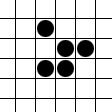
\includegraphics[height=3cm]{glider.png}
\end{center}
If we lived in the game of life, then we could completely describe the state of
the world by listing which cells are on or off.
The universe may contain nothing but gliders, yet we still have no need
for the idea of a glider to describe everything in it.
The glider idea is at once useful, created, and dependent upon minds for it to
exist.
There is nothing false about discussing gliders, but gliders are not an
intrinsic part of the world.

And here's why I'm discussing all of this:
\begin{obs}\label{o3}
    Truth is a useful fiction. It is an invention, and not a natural part of the
    world.
\end{obs}

This observation disagrees with the common intuition from claim \ref{c7} that
truth is independent of minds. How can I justify observation \ref{o3}?

\begin{argt}[That truth is an invention.]\label{a2}
    \normalfont
    \begin{itemize}
        \item[]
        \item
    The idea that ``$x$ is true'' only makes sense as a denial of the opposite
    idea that ``$x$ is false.'' If there were no concept of a false idea, then
            there would be no use or meaning in considering true ideas.
        \item
            The idea of falseness is clearly invented. We can describe
            the world without having to include the idea of falseness.
            There is a purpose to the idea of falseness, which is to understand
            mistakes or deception.
        \item
            Since the idea of truth is essentially paired to the idea of
            falseness,
            it must be the case that both ideas are invented.
    \end{itemize}
\end{argt}

A natural counter-argument is that perhaps falseness is invented while truth is
not.
I will expand on this point below in \S\ref{s_mental_words}
by looking more closely at the dependence between ideas that are alternatives to
each other.

\section{What Ideas Are}

In order to better understand the relationships between alternative
notions (up vs down, red vs orange, true vs false), it's
helpful to explore the question:
\begin{question}
    What kind of thing can be true or false?
\end{question}

So far I've been blithely using the words {\em idea} and {\em concept} to talk
about things that might be true.
As a reminder, the word {\em idea} in this article is adjusted to focus on
clear and meaningful expressions that can be true or false.
So when I say {\em idea}, I'm excluding
things like ``the idea of the color green'' because that isn't something that
could be true or false.

Some philosophers go into a tizzy when you ask this question (question 4).
You might say a grammatically correct {\em sentence} can be true or false,
but then you must deal with any random yet grammatically correct string
of words
like ``a yellow sadness confused the used
passenger;'' or logical ambushes like ``this sentence is false.''
There's a deceptively deep rabbit hole here that I don't want to get stuck in.

Instead of trying to find a perfect answer, I'm going to speak at a high level
and suggest two connections that help us better understand the word {\em idea}
as it's used in this article.
I am {\em not} going to define exactly what an ``idea'' is.
I'm going to keep the word {\em idea} as a placeholder for our
intuitive understanding of what can be true or false, and I'll analyze some key
properties of this intuitive notion.
% TODO XXX ^^^ Do I make use of this last sentence?

\subsection{Questions and Answers}

The first connection I want to make is between ideas and answers to questions.

If an idea tells us some information, then it must distinguish between different
possibilities. If I say ``I'm having a nice day,'' then I'm distinguishing this
from the possiblities of having an astounding day or a dog-tired day.
If there were no other possibilities,
then there is no information conveyed. If I said
``red is red,'' without context, then it's confusing because it's not clear what
alternative I'm excluding.

There's a nice mathematical analogy here. It's almost as if there were a short
conversation like this:
\begin{itemize}
    \item{} [Mathematician A] I know $x\in X$, but what is $x$?
    \item{} [Mathematician B] Oh, it turns out that $x=4$.
\end{itemize}
There is a question (what is $x$?) with a set ($X$) of possible answers. The
information content --- the idea being expressed ---
is an answer to this question ($x=4$). If you say ``my name is Inigo,''
then you are answering the implicit question ``what is your name?'' whose set of
possibilities is the set of all names.

This mathematical analogy is not perfect.
Since we often think about what we say without thinking carefully about the
alternatives, the question we're answering
is typically implied, and may not be clear, even to
the speaker. I claim that if you {\em did} stop and think about any statement
you
make, then typically you'll be excluding some specific alternatives
(occasionally you may say things that don't have much information, and are
correspondingly not excluding anything, as in ``red is red'').
Another imperfection with the analogy is the fact that mathematical
sets are well-defined objects, and we often don't have full awareness of the
alternatives for an idea.
If I say ``I'm 10 years old,'' then the set of ages is understood
to be non-negative integers; that's mathy. If I say ``this wine tastes of
elderberries and the phlegm of an incontinent camel,'' then we must admit there
seems to be a fuzziness to the set of things a wine can apparently taste like;
you'd be hard-pressed to enumerate this set exactly.

Nonetheless, the analogy helps us to build our intuition.
An idea has meaning only because it expresses one way things
{\em are} from amongst a
(non-mathematical) set of possible ways things {\em could be}.
Similarly, a question is an expression of a set of possible ways things could
be, along with a desire to learn which item in that set is correct.
I'll summarize this
connection as:
\begin{answer}{4}
    An idea is an answer to a question.
\end{answer}

This is similar to a definition, but really I'm just breaking down
one intuitive notion (ideas) into two other not-carefully-defined notions
(answers and questions). I still find this connection useful, as we'll see
below.

\subsection{Goals}

The second connection I'd like to make is inspired by asking:
\begin{question}
    Why do we ask questions?
\end{question}

Every idea we express or deliberately think about is motivated by a goal.
If we express an idea, that is an action we're taking,
and conscious actions are
goal-based.
Some ideas occur to us unbidden, as in perceptions of the world,
thoughts expressed by others, or associations evoked from something outside of
our own thoughts.
Those sources of thought, all of which are external, don't need to be
goal-based.
Yet when we take one of these external notions and then build
ideas atop them, then our added ideas are goal-based.

I think so because any thought we consciously create --- that is,
thoughts which do not arise externally --- are a kind of action
we choose to take. I'll call these {\em internal ideas} to
distinguish them from external notions (like perceptions or ideas
communicated by others).

You might raise an objection at this point by thinking of cases where
an action or internal idea does not seem to arise from a particular goal.
For example, what if someone tells you to ``say $x$'' where $x$ is a statement,
and you say it? It may seem that you had no goal in mind in saying $x$.
In this case I'd say your goal is to respect the relationship you have with the
person who told you to say it. If they're your teacher, then you may want to
learn from them (this is a goal), or you may simply want to avoid the
awkwardness of ignoring your teacher in front of your peers (another goal).

You might think of other examples, such as a child playing, or a person who
stops what they're doing to indulge their curiosity. In these cases, I'd say
that play is for fun (a goal), and that curiosity itself is a goal --- indeed, I
see curiosity as a fundamental drive of human behavior, along with hunger and
fear. You might also say that some actions like sleepwalking, or a muscle
reflex, are not goal-driven. In this case I would agree, but I'm excluding those
kinds of actions by saying that {\em conscious} actions are always goal-driven.

Based on this, we can have conscious thoughts that are ideas, and others that
are questions. The perspective of this paper is that an idea is an answer to a
question, so in either case there is a question present. And a question is a set
of possibilities along with a desire to know which of these possibilities will
help us move toward our goal.
Let's summarize this as:
\begin{answer}{5}
    Every question we consciously consider is motivated by a goal.
\end{answer}
This includes both questions we ask directly as well as
implicit questions that give meaning to a conscious idea as per
answer 4.

\subsection{Impossible Ideas}

What I've argued is that every idea is an answer to a question, and that every
conscious question is motivated by a goal. Putting these two together,
{\em every
internal idea is connected to a goal}. I've used the word {\em internal}
to exclude things like perceptions which don't need to be associated with
conscious questions.

This is a powerful claim. One key implication is that we cannot even think of
internal ideas (again, excluding things like perceptions)
that are not motivated by
a goal.

It's possible that the goals that first led us to an idea are
different from the goals we later associate with it. For example, we may first
think of a water heater as a way to make tea, and later learn how to make
instant ramen with that same water heater.

It's interesting to see an example of an idea we {\em cannot} think of.
Consider learning to speak Mandarin when you only speak English.
This is difficult because Mandarin uses {\em tones} --- patterns in the pitch of
your voice --- as a key part of a word's pronunciation.
Two words in Mandarain can have
the same consonant-and-vowel sequence, yet be
pronounced differently based entirely on their tones.
English-only speakers typically have no concept of a tone because there was
never any reason for them to form this idea.
They've learned to understand the consonant-and-vowel sounds in English, and to
ignore other points of data from word sounds. If we imagine a world without
tone-based language, then we can imagine that people would never think of
tones at all.

This isn't a perfect example of an idea we can't think of --- because we {\em
can} think of it; it's just an unknown concept for some people.
It's not my fault I
gave a partial example.
It's literally impossible for me to express an idea that
cannot be thought of.
But such ideas must exist because we'll never
have experienced all possible goals.
For every goal we never think of,
there is the question of how to achieve that goal, and an answer to this
question. We will never think of any of these ideas.

If it helps your intuition, consider an alien race that sees colors we cannot;
their eyes see different wavelengths than human eyes.
They will have many words for ``colors''
that we would not recognize as colors. These colors are another kind of notion
we almost cannot think of.
Again, technically, this example is
partial (hence the word {\em almost})
because scientists can understand what I mean --- and, again, any
example I actually give must necessarily be partial. But if you can stretch your
imagination a bit in thinking of these aliens as having entirely new dimensions
of perception, and we never meet these aliens or encounter this dimension of
perception, then you can imagine ideas that we will never think of.

% XXX Add some kind of callout to this subsection to summarize and highlight the
%     main point of it. Or does it go in the next subsection?

\subsection{Mental Words}\label{s_mental_words}

We have the rough workings of a model of human thought.
I'll add one more
ingredient to this model.
Earlier, I said that this articule adjusts the meaning of the word
{\em idea} to exclude, say, the color green since a color
can't be true or false.
In this section I'll introduce the term {\em mental word} to talk about
things like colors;
mental words are
the pieces that ideas are made of.
They include things like
colors or water heaters or letters of the alphabet.
Intuitively, if
ideas are {\em mental sentences}, then mental words are whatever building
blocks these sentences are made from.
As with the term {\em idea}, I won't try to define mental words,
but I will analyze our intuition around them.

To ensure the notion of a mental word is clear, let's consider another example,
besides {\em green}.
Suppose one day you're stung
by a distinctive-looking wasp.
A year later, you see a similar wasp, and you
steer clear of it, remembering the sting.
It's not that you have an actual word you can say out loud to name this wasp,
but still you have a connection in your brain that can recognize it and
understand something about it.
Contrast this level of awareness to a bug you may peripherally perceive, but
never care about; if you saw such an innocuous bug later, you would have no
associations at all with it.

Perhaps mental words originate in a brain process that precedes conscious
thought.
I'm not going to suggest a specific origin story for mental words
because we don't need
to in order to say something interesting.
Above, I argued that any internal idea is a conscious action, and therefore is
goal-motivated. The first time we use a mental word consciously, it will be a
part of an internal idea. In other words, as soon as we deliberately
(consciously) think of a mental word, it is attached to a goal, and this
attachment is unavoidable.

I'll summarize this idea along with the previous section as:
\begin{obs}\label{o4}
    Any thought we consciously create is goal-based.

    \medskip

    That is, it's impossible to think of an idea or mental word which is
    truly goal-free.
\end{obs}

Here's a diagram summarizing the mental model of ideas used in this
article:

\begin{center}
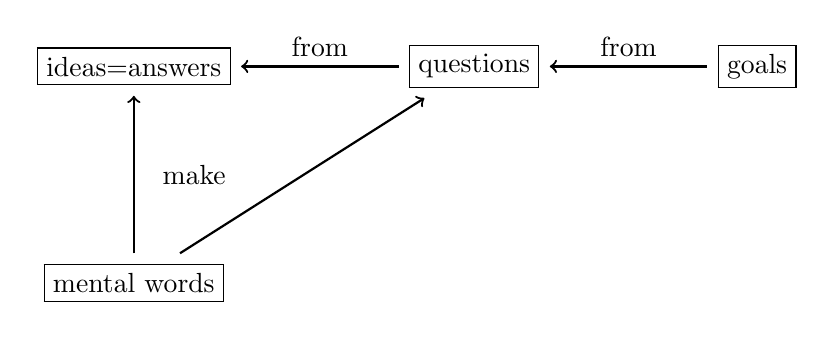
\begin{tikzpicture}[node distance = 2cm, thick]%
    \node (1) {\fbox{ideas=answers}};
    \node (2) [right=of 1] {\fbox{questions}};
    \node (3) [right=of 2] {\fbox{goals}};
    \node (4) [below=of 1] {\fbox{mental words}};
    \draw[<-] (1) -- node [midway,above] {from} (2);
    \draw[<-] (2) -- node [midway,above] {from} (3);
    \draw[->] (4) -- node [right] {\ \ make} (1);
    \draw[->] (4) -- node {} (2);
\end{tikzpicture}%
\end{center}

In this diagram, I've included the notion that mental words make questions as
well as ideas. This makes sense because a question is the same thing as an idea
with a blank space in it: {\em what is your name?} is the same as
{\em your name is $x\in X$?} where $X$ is the set of possible names.

A mental word can only add information to an idea by distinguishing the idea
from alternatives.
There must be possible variations of the idea that are excluded.
This set of variations might not be clearly defined;
if I asked why the chicken crossed the Mobius strip\footnote{Answer: To
get to the same side.\par Note that the corresponding idea {\em The chicken
crossed the Mobius strip to get to the same side} seems to pertain to a new
kind of truth not discussed in this paper ---
a kind of ``truth'' based on comedic
value, albeit rather hypothetical value in this case.}
the set of possible answers allows for creativity, and is not something we could
easily enumerate.

Some pairs of mental words, like {\em light} and {\em dark}, are essentially
always understood as alternatives to each other.
Questions like ``Is idea $x$
correct?'' will typically have possible answers {\em true} or {\em false}.
Some mental words depend upon specific variations to have meaning.
Heat makes no sense without cold; nor does light without dark.
In this way, the notion of truth cannot exist alone;
it is one with the notion of falseness. This interdependent
coexistence bolsters argument
\ref{a2} above that truth is an invention.

Some questions seem less useful than others because we can easily guess their
answers. Imagine asking about a random person ---
are they less than 110 years old?
We have mental words for age groups like kids,
toddlers, and teens, but we don't have a name for people under 110;
that mental notion is less useful.
There is a golden zone of balanced ignorance in which questions and their
corresponding mental words are most useful, and therefore have
the most potential to be {\em effectively} true. It's worth taking a closer look
at the relationship between truth and ignorance.


%
% NOTE
%
% The one-word proof that truth is not the bedrock of human knowledge:
% hello
%
% Probably rephrase this particular claim to match the proof, but what I mean is
% that we understand actions as more fundamental than truth-bearers.
%
% Slight elaboration: Not everything we do is an idea. Anything we do with an
% idea is an action, but not all actions are things we do with ideas. Actions
% precede ideas in a hierarchy of the human experience.
%


\section{Ignorance and Omniscience}

Truth only makes sense in the presence of ignorance.
% TODO XXX Add a bit more of an intro to this section after I've written the
%          rest of it.

\subsection{The Role of Ignorance in Truth}

I'll use three example questions
to help build up an intuition about the role of
ignorance in ideas and truth.
To state these questions, I'll define a
{\em pleven} number to be an integer which is neither even nor odd. Spoiler
alert: there are no pleven numbers. But, if you squint a bit, you can imagine
they exist. This strange thought experiment is purposefully awkward, and we'll
explore the awkwardness behind it.

Here are three questions:
\begin{enumerate}
    \item[{\bf Q1.}] How long will my commute be this morning?
    \item[{\bf Q2.}] What's the first positive pleven number?
    \item[{\bf Q3.}] What would the color blue be if it weren't blue?
\end{enumerate}
Question {\bf Q1} seems practical enough. At first glance, there do not appear
to be any strange assumptions behind this question.
Question {\bf Q2}, on the other hand, feels weird because we're asking about
something that doesn't exist. How can we answer a question of detail about a
nonexistant thing? Question {\bf Q3} seems to go one step further in this
direction, almost making no sense unless we decide to think poetically or
playfully, giving up on taking ourselves literally.

Now, for a moment, imagine that you have complete and immediate awareness of all
commute times. Suddenly question {\bf Q1} seems silly, a bit like ``Is 3
divisible by 3?'' because the answer is obvious to you.
Depending on how profoundly
familiar you feel with commute times, question {\bf Q1} may even feel to you
like ``Is blue blue?'' which is so obvious as to be confusing. If you force
yourself to take seriously the question ``Is blue blue?'' then you're in the
same mental space as question {\bf Q3}.

Returning to a human who doesn't know all commute times,
question {\bf Q1} is
reasonable because we can imagine worlds with different commute
times. This kind of imagination is akin to ignorance --- to not knowing the
answer.
The other questions are strange because we're deeply familiar with the state of
the world that gives the answers. We can't easily imagine pleven numbers
existing, or blue not being blue.
I included question {\bf Q2} to show how a question's status depends on the mind
considering the question. A kid just learning about even and odd numbers will
take this question seriously --- it makes sense to them. But it stops making
sense once you realize there are no pleven numbers.

\iffalse
For us mere humans, why does question {\bf Q1} seem completely reasonable while
question {\bf Q2} seem strange and question {\bf Q3} seem nonsensical?
The answer depends on our internal model of the world. For commute times, we can
easily imagine the answer being many different values. It feels like we don't
know ahead of time what it will be.
Yet for the other questions, it's difficult to imagine worlds where an answer
makes sense.

If we were to ask question {\bf Q2}
to a young kid --- someone who could understand the
definitions involved, but hadn't thought about things carefully yet --- we can
imagine that the question makes sense to them. Question {\bf Q2} is one that
at first seems reasonable, and later seems silly after we know pleven numbers
don't exist. In a sense, all questions are like this. That is, all questions
make sense {\em only} when we can imagine that other answers are possible.
\fi

I'll summarize this line of thinking as:
\begin{argt}[That ideas only make sense in the presense of ignorance.]
    \label{a3}
    \normalfont
    \begin{itemize}
        \item[]
        \item Every idea is an answer to a question.
        \item A question only makes sense if we can imagine that more than one
            answer is possible.
        \item When we're deeply familiar with the state of the world that
            determines the answer, the question no longer makes sense.
        \item Therefore, questions --- and their corresponding ideas --- only
            make sense when they are about things we don't know, or can easily
            imagine that we don't know.
    \end{itemize}
\end{argt}
This is a refutation of true ideas being independent of minds (from
claim \ref{c7}). Ideas themselves need the ignorance of minds before they can be
conceived as meaningful.

% TODO XXX Eventually provide an Observation environment that fully refutes
% claim 7, or whatever refutation thereof I feel comfortable with.
% I like the principle that the key claims of this article are highlighted
% nicely in observation brackets.



% One resulting argument is something like if we knew the answer, we would not
% understand the question. In this way truth is dependent on minds.
%
% I think to refute the other side of claim 7 is another place. Some things,
% like 1+1=2, just feel true no matter what. BUT the more interesting truths to
% us are those that we feel more unsure of. We have a hypothetical model of the
% world in our mind, and we don't know for sure how everything works. We imagine
% that if we take action A, we get result A; B->B, etc.
% Any generalization of an idea, any concept of a pattern,
% is based on the imagination that reality could
% have been any other way. If we live in Conway's game of life, then we think
% understanding the rules is meaningful, but in some sense it's no better to
% know the rules than to know all of history. 
%
% I think what I'm leaning toward is something like: We will almost always end
% up with "bad reasoning" like "red bowling balls are lucky." But it's not 100%
% bad reasoning. It's more like, the reasoning will typically be bad when we are
% in areas of high uncertainty. The least assumptive idea is something like if I
% do action A in exact context C then I get result B.
% But for this to be re-usable we necessarily need context C to be changing --
% at very least, eg, we want the timestamp in C to be different. I'd also argue
% that we don't know how to preserve other aspects of the context. An analogy
% could be not knowing which basis is meant in a vector space when we change
% "only the y coordinate;" we could think in terms of an ideal gas law, or in
% terms of asking patients to eat fewer bananas.
%
% I'd say that in situations where we are learning the most, that we also have
% the least understanding of the other variables to control for. How can I argue
% for exactly this? If something is reliable, then we understand it well, and we
% don't think about it much. I don't worry much about addition of small numbers,
% or about quantum physics when playing pool. But there are many problems where
% I have many unknowns. When I raise my kids, how often should I let them take
% small risks? How can I help them see that sugar consumption is not healthy
% despite their lack of maturity and the deliciousness of sugar? These are
% realistic and challenging goals, and it's tricky to even know all the
% variables. Another example might be choosing a nutrition plan, or designing a
% physics experiment.
% 
% Iteration:
% Suppose determinism. If not, then either we have no influence over the outcome
% - nothing to learn - or it's a probability distribution, in which case we can
%   consider the probability of a good outcome as the outcome itself, and then
%   we're back to determinism.
% If there were truly only one variable in a repeatable setup, then it's
% actually not very hard to learn. Why not? Technically, it could be quite
% complex, such as effectively having many different variables encoded into a
% single variable. But then this feels like it's not truly one variable. So for
% the term 'single-variable' to be useful, I think what we mean is an outcome
% that is something like "mostly absolutely continuous" in terms of the input.
% To be a mathematician, I'd say piecewise absolutely continuous where the
% number of pieces is not too large. Then we can do a few experiments and
% typically we will understand the relationship completely. The more variables
% there are, the harder the problem is. The questions we care most about are the
% ones with interesting goals but that are challenging. And in these cases, the
% context is critical. Attached to this argument is the idea that if we
% literally controlled for all variables except for one, then we would be
% limiting ourself to a single experiment (time is a variable, and even if not,
% we'd require a reset of the entire world).
%

\subsection{Omniscience}

I'll briefly describe a thought experiment that can be illuminating.
It shows XXX WHAT IT SHOWS

The aim of the thought experiment is to imagine that you know everything,
and that you know it so well that a question about the world feels like ``is
blue blue?'' in that the answer seems self-evident to you. This is a bit
different from knowing the axioms of math and being asked if a certain theorem
is true --- in that case you would have enough information to derive the answer,
but you'd have to think about it first.

To solidify the thought experiment, pretend the world is a single instance of
Conway's game of life. Any time step is a 2D grid of cells that are on or off.
Visualize a 3D version of this where each slice is a single time step. In this
way, all of timespace is laid out before you as a single static object. Time is
no longer a mystery, but rather a dimension just like space.

Hence you ``know everything'' in the sense that you know the full physical state
of the world. Perhaps you don't know all possible mathematical truths, or all
other possible worlds. So this is a certain kind of omniscience. Let's call it
{\em physical omniscience}.

Now someone who isn't omniscient points to a glider at a certain time step, and
they ask how long this glider will live. You, being omniscient, respond:
``What's a glider?'' There's no reason for you to know or care about what a
glider is because you can see all of history without that concept. Once you
learn what a glider is, then you can easily answer the question. But such a
question feels arbitrary to you, in that a questioner has defined some
random-seeming idea and asked a question about this idea in a situation where
the answer is inevitable. It may feel as if someone defined even and odd
numbers, and started to go through all the primes checking to see if each one
were odd and even. It feels like a silly task when you know that 2 is the only
even prime. But it doesn't feel as useless before you know that.

Let's summarize this idea as:
\begin{equation}\label{eq1}
    \text{\em Physical questions seem nonsensically obvious to the physically
    omniscient.}
\end{equation}

Now let's imagine that you are both physically omniscient, and that you identify
with one particular agent in the world.
When you see this agent in the world you
think ``hey, that's me!'' What kind of goals might you have for this agent? I
don't think you can have {\em any} goals, because you see before you the
full life of your agent just as you see the indelible ink on a page. To imagine
a different path is to reread The Lord of the Rings and hope that Gollum
becomes an insurance claims adjuster by the end. If you're creative, you may
choose to ignore what you already know, but your rational mind understands the
futility:

\begin{equation}\label{eq2}
    \text{\em The physically omniscient are not personally motivated by
    physical goals.}
\end{equation}
 
I say {\em physical goals} to tease out other goals that we can imagine, such as
proving a mathematical theorem. We may also imagine that you, the omniscient
party, exist in some outer world, outside the confines of the world you have
omniscience about (think The Matrix).
You might have agency in this outside world, but the point of this thought
experiment is to look at how knowledge of {\em our} world affects ideas {\em
about our world}, not about other words. This relates to (\ref{eq2}) in that my
phrase {\em physical goals} are restricted to actions and results observable
within our ``inner'' world, then one that you know all about.

When you know the full physical state of the world, it's
like listing all possible worlds $\{x_1, x_2, \ldots\}$ in a giant list, and
then learning which possible world is the real one. When you're omniscient, you
know there's a certain number $k$ that indicates the real world $x_k$.
If the world used the game of life as the rules of physics, then perhaps this
number $x_k$ would be the starting conditions of the world; everything else
follows. No matter what the rules of physics are, we can suppose there is some
way to encode the state of the universe across all time, and the number
$x_k$ can be this encoding.

Building on the idea of encoding the world in a single number,
I'm going to pose a strange-seeming mathematical question whose purpose is
(a) to show that some math questions make us wonder what the
point of the question is, and (b) to point us toward understanding the role of
curiosity and abstract thought in our thoughts.

Given any positive integer, I can write that number in base 2, in base 3,
etc.\footnote{We normally write a number, like 7, in base 10 because we have 10
fingers, and 10 digits (0-9). If we had only, say, 5 fingers, then we'd have
digits 0-4 and we'd count like this: 0, 1, 2, 3, 4, 10 (this means 5 to us), 11
(meaning 6), 12 (meaning 7), etc. Base $b$ notation is how we'd write numbers if
we had $b$ fingers instead of 10. If this notion is entirely new to you, it's
too much to learn in a footnote, and I recommend googling ``introduction to
number bases'' to learn more.}
I'll create a table by writing a number's binary (base 2)
form in the top row,
and then below that its base 3 form, then its base 4 form, and so on, keeping
them all right-aligned. Here's a table for the number 534:

\begin{center}
\begin{tabular}{cccccccccc|c}
  &   &   &   &   &   &   &   &   &   &\em base \\
1 & 0 & 0 & 0 & 0 & 1 & 0 & 1 & 1 & 0 & \it 2 \\
  &   &   &   & 2 & 0 & 1 & 2 & 1 & 0 & \it 3 \\
  &   &   &   &   & 2 & 0 & 1 & 1 & 2 & \it 4 \\
  &   &   &   &   &   & 4 & 1 & 1 & 4 & \it 5 \\
  &   &   &   &   &   & 2 & 2 & 5 & 0 & \it 6 \\
  &   &   &   &   &   & 1 & 3 & 6 & 2 & \it 7 \\
  &   &   &   &   &   & 1 & 0 & 2 & 6 & \it 8 \\
  &   &   &   &   &   &   & 6 & 5 & 3 & \it 9 \\
  &   &   &   &   &   &   & 5 & 3 & 4 & \it 10 \\
\end{tabular}
\end{center}

I can make such a table for any number.
I can further imagine that each number in the table is the value of a cell,
analgous to the cells in the game of life being on or off.
I can think of the
top row as the first time step, and as each subsequent row as the next time
step.
(Notice how the number 534 effectively encodes and captures this entire
world; this is ``world 534'' in some sense.)
Now I can ask a question like:
{\em How long does the 1 in the second-from-right column survive?}
In other words, how long does this particular cell:
\begin{center}
    1 0 0 0 0 1 0 1 \fbox{\bf 1} 0
\end{center}
remain as a 1 in the rows immediately below the top row?
The answer, for 534, is that this value survives for the first 4
time steps.

As promised, I hope that you have two reactions to this question, corresponding
to earlier goals (a) and (b) of this thought experiment:
\begin{enumerate}
    \item I hope you find this question to be arbitrary. How is it useful, or
        why would we ever ask this question outside of a philosophy paper?
    \item I hope you wonder:
        Out of curiosity, are there any fun mathematical patterns to questions
        like this?
\end{enumerate}
For a moment, I'm going to ask you to pretend that you don't have any curiosity,
so that the first reaction --- wondering why we're doing this --- is your only
reaction.

But now consider the similarities between these questions:
\begin{itemize}
    \item{} [In reality] How long will this person live?
    \item{} [In Conway's game of life] How long will this glider live?
    \item{} [In a number base table, as above] How long will this value survive?
\end{itemize}
These questions all have the same shape: They are noticing an
object in the world, and are asking how long it will be around.
We probably have different emotional reactions to the questions, but they feel
like the same kind of question to the physically omniscient.

If you asked how long you have to live to the physically omniscient, they can
answer your question, but it feels like a pointless question to them. I've
purposefully chosen a clearly-motivated-to-mortals question (how long will I
live?) to help illustrate
that no amount of motivation can really cross the gap from ignorance to
omniscience. I'll summarize this idea as:

\begin{equation}\label{eq3}
    \text{\em Mental words seem arbitrary and unmotivated to the physically
    omniscient.}
\end{equation}

The idea of {\em curiosity} throws a wrench into this simple perspective because
virtually any question that can be asked can be motivated, in theory, by
curiosity. If you're physically omniscient and curious, you might find all
questions to be motivated.\footnote{I suspect curiosity has an evolutionary
origin that connects it with survival. For example, perhaps a curious pre-human
primate would discover the utility of controlled fire, whereas a less curious
species would not. This paper won't try to analyze curiosity, but I think it's
something we could analyze and put boundaries around. We humans find some things
more interesting than others, and there are probably ways to understand this.}

One thing we can do to fit curiosity into this model is to consider two kinds
world: the physical world, and the world of abstract thought.
A historic fact is an idea about the physical world, while a mathematical
theorem is an idea about the abstract world.
Many ideas blend these two worlds together, such as asking if a particular
theory of physics is true. In that case, we imagine a possible world based on a
physical model; this model lives in the abstract world. And we ask if this model
is a good approximation for reality; we can do a physical experiment to check.

Whenever curiosity is the motivation for a physically omniscient person, there
must be an abstract mental word involved. If there were not, then there is
nothing unknown that makes sense as a question --- we get back to
``is blue blue?'' which invokes no curiosity. And once we're looking at abstract
notions, then we're outside the realm of physical knowledge.
If we wanted to, we could change the thought experiment to imagine a person who
knows all physical states of the world {\em and} all abstract ideas as well. I
think that such a person would then be incapable of curiosity, as no question
could possibly motivated. Indeed, all questions would seem nonsensically obvious
to such a being. Sounds like a disappointing existence.

I'll summarize the ideas of this section and the previous one as:
\begin{obs}\label{o5}
    We have no motivation for ideas or mental words without ignorance about
    them.
\end{obs}

The omniscient thought experiment also leads as to another argument that truth
is an idea we created for a purpose:

\begin{argt}[That truth is an invention]
    \label{a4}
    \normalfont
    \begin{itemize}
        \item[]
        \item If we can fully describe the phyiscal world without
            mental word $x$,
            then $x$ must be created by us.
        \item We can only create mental words if we have a purpose for them.
        \item So if mental word $x$ is not needed to fully describe the
            physical world, it must be invented.
        \item The notion of truth is not needed to fully describe the
            physical world.
        \item Therefore truth is an invention.
    \end{itemize}
\end{argt}

One response to the above argument is that basically everything would then count
as an invention. For example, suppose we can explain the universe entirely in
terms of atoms. Then we do not need the mental word for rocks, and rocks would
count as invented!

I agree that this argument shows the word {\em invention} is being used quite
differently from the usual term in the English language. At the same time, I
think there is something correct in saying that the notion of rocks was
invented. If an omniscient person saw two gliders, they would have no motivation
to say they are ``the same thing,'' noticing something in common with the
configuration of cells. Similarly, we as humans are adding a new idea to the
world when we look at two different rocks and call them ``the same thing.''

The particularly interesting thing about argument \ref{a4} is that truth feels
like the bedrock to human thought. The notion of truth feels akin to the notion
of an atom in physics. But it cannot be, for there are things we must understand
before we understand truth.


% TODO Ensure I clarify that I use the word _notion_ as a synonym for _mental
% word_.

\subsection{Dependence on Context}

Argument \ref{a1} showed that 
the definition of effective truth matches our
intuition for truth.
Since then,
we've been exploring how ideas only make sense to us in the
presence of both our ignorance as well as our goals.
With effective truth in mind, I want to look again at
the relationship between truth and our limited understanding of the
question behind an idea.

Suppose a question is an easy one. For example, consider the addition of small
numbers. This feels like a solved problem because anyone with enough experience
will essentially always get the correct answer.
Juxtapose this with a problem that seems more difficult, like predicting the
stock market. When it comes to predicting stock prices, even experts will make
mistakes on a regular basis.

Behind every question is a goal, which --- for effective truth --- gives
us a way to test ideas.
We can think of a goal, or a test for a goal, as having some inputs
and some outputs. For addition, the inputs are the two numbers being added, and
the output is their sum. For stock market prediction, the input is everything
that influences the stock market,
and the output is how much
money you make or lose.
To be clear, I'm thinking of tests as being deterministic once we know enough
about the inputs. If something seems like a probability, such as whether it will
rain tomorrow morning, then it simply means we have not accounted for all
of the variables. It may be difficult or even impossible for a human to know all
the variables, so the claim is not about how a human brain works, but rather
about how the world works. Fix the inputs, and the outputs are certain.

When a question has a simple relationship between inputs and outputs, then the
corresponding truth --- such as how to add numbers --- feels easy. Complex
input/output relationships make the corresponding truths feel difficult.
When a problem feels easy, it becomes less interesting to us.

In some special cases, such as in pure mathematics,
we have awareness of all the variables that might affect an outcome.
In most cases, though, we don't.
When we don't know all the variables relevant to an idea, then each time we
test the idea, there are elements of the test we don't control for.
This makes the efficacy --- the truthiness --- of an idea dependent on the
variables we don't control for, that is, the context.

I'll summarize this as:
\begin{obs}\label{o6}
    Many ideas that aim to achieve an outcome don't account for all the inputs
    that determine if the outcome is reached or not. There are exceptions, such
    as in mathematics.

    For the many ideas that don't account for all relevant inputs, whether the
    idea achieves the goal depends on the context in which we apply the idea.
\end{obs}

To help build more intuition for this, consider the idea that water boils at
100\degree C. For most of us, this is a simple truth we can use in our daily
lives. However, at different air pressures it is no longer accurate. Even a
truth as scientific and practical as this is dependent on additional context.

A counterargument to observation \ref{o6} goes like this:
It's true that sometimes an idea like ``water boils at 100\degree C'' misses
some important context --- but we can always fix the idea by adding in the
missing context, such as accounting for air pressure.
Technically, I think this point is true, but the gist of the observation is that
many of our ideas implicitly make assumptions about their context. It seems
wrong to completely discard the idea that water boils at 100\degree C because,
for many practical purposes, it's effectively true. Philosophically, we are
forced either to say that
basically everything you think you know is now
declared as completely false, or to accept that much of what we consider to be
true is only provisionally true.
The perspective of this article is not to redefine truth, but to analyze the
intuitions we have and to be honest about the role truth plays in our lives.
Hence, given the above choice, I'll say that ``water boils at 100\degree C'' is
provisionally true rather than false.

Recall that claim \ref{c7} outlined our tendency to think of true ideas as
independent of minds and not depending on context. With observation \ref{o6}, we
have largely refuted those ideas.
True ideas require minds to make sense.
Without the ignorance of minds, questions do not make sense.
Without the goals of minds, ideas are unmotivated.
And without full contextual awareness, our tests of ideas are noisy ---
whether the test succeeds depends on things we have not accounted
for.

\section{The Fuzzy Edges of Ideas}

If there is a theme to this article, it's that truth isn't as
objective and absolute as we usually consider it to be.
Along those lines, let's
look at another intuition we tend to have about truth.
Consider the question:

\begin{equation}\label{eq4}
    \text{\em Given two specific animals, are they members of the same
    species?}
\end{equation}

At first glance, this appears to be a perfectly reasonable scientific question
that ought to have a clear yes or no answer. If I point to two people, the
answer is yes. If I point to a dog and a cat, the answer is no.

The mental word {\em species} carries with it a sense of clarity and a
sense of being intrinsic to the world.
This section will consider
these proposed two properties of mental words:
\begin{enumerate}
    \item{} [The Clarity Property]
        If a person fully understands the mental word $x$,
        then they can always know if thing $y$ is an $x$;
        the distinction is clear.
        Example: Is an apple a fruit?
    \item{} [The Intrinsic Property]
        When we learn a mental word, we are learning about the way the world
        is --- we are not deciding anything about the world, but observing it.

        Example: It seems silly if I point to a water molecule and ask if we got
        the definition of water wrong, and maybe we should redefine {\em water}
        to exclude this one molecule.
        Liquid H$_2$O is water, and this notion is part
        of nature, not something I decided.
\end{enumerate}

% TODO: I'm thinking maybe I ought to replace "mental word" with "concept". It
%       might simplify and clarify the article.


% Now I'm thinking that it makes sense for arbitrariness to build AFTER
% fuzziness because some of the arbitrariness can creep in at the edge cases.

% HERE: Next up, talk about the fuzzy edges of mental words.

\subsection{Most Mental Words Are Fuzzy}

Let's take a closer look at question (\ref{eq4}), whether two animals are of the
same species.

Traditionally, a species of animals is defined as the largest group of animals
which can reproduce together. But this idea doesn't always work the way we want
it to. A simple challenging case occurs when a group of similar animals
reproduces asexually, with a single parent resulting in two copies of itself. In
this case, we cannot use the above definition, and must begin looking at
features of the animal itself. Yet the features itself can be surprisingly
tricky to work with. For example, chihuahuas and Great Danes are the same
species, while jaguars and leopards look similar yet are different species.

In fact, the closer we look at the notion of a {\em species}, the more problems
we reveal:
% HERE List problems like: microspecies, hybridization, ring species, evolution
\begin{itemize}
    \item{} [Microspecies] Scientists have found that what you intuitively
        think of as blackberry plants are actually a
        collection of approximatedly 400
        different species that are quite similar to each other.
        Species within such a group are called {\em microspecies}.
        Most people would think of two such plants as the same species,
        but scientists disagree.
    \item{} [Hybridization] A mule is the offspring of a horse and a donkey;
        horses and donkeys are considered to be different species.
        Mules are thus a {\em hybrid}, a cross between species.
        Mules
        are typically unable to reproduce, which means the
        traditional idea of a species would not apply to them.
    \item{} [Ring Species] Different communities of a bird called the
        {\em greenish warbler} live in subgroups around the Tibetan Plateau.
        Many of these communities that live near each other can interbreed, but
        the most disconnected groups cannot. We have
        communities of similar animals --- call the groups $A$, $B$, and $C$ ---
        where $A$ and $B$ can interbreed, and $B$ and $C$ can as well, but $A$
        and $C$ cannot. This setup is called a {\em ring species}, and reveals
        another challenge to the reproduction-based definition of a species.
    \item{} [Evolution] Finally, we have to take into account the idea of
        evolution itself.
        Given two same-species parents and their offspring, we see the
        offspring as belonging to the same species.
        But if we extended this line of
        species labels throughout the complete family tree, we'd end up naming
        many living things as the same species, despite vast differences.

        For example, the human precursor species {\em homo habilis} is
        thought to have evolved directly into {\em homo erectus}.
        If we take the idea of a species seriously,
        then we are forced to believe in a family
        with two homo habilis parents and
        the first-ever homo erectus as their offspring.
        Yet there would be no enormous
        change within this particular family.
        It's simply a line we force
        ourselves to draw to be coherent.
\end{itemize}

The idea of a species is not really about the ability to make
offspring together.
That traditional definition is useful for the many cases in which it
makes sense.
But it is trying to capture an
intuitive notion for a {\em species} that is
based more on ad hoc practicality than on a single guiding scientific principle.

The notion of a {\em species} is fuzzy --- it's not a mathematically elegant
concept, but rather a pragmatic one with unclear edge cases.

And the fuzziness of a {\em species} is not alone. While {\em fruits} can be
defined as edible plant structures associated with seeds,
{\em vegetables} have no such botanically-based definition.
It's true that vegetables are typically edible parts of plants,
but not every edible part of a plant is a vegetable;
apples aren't vegetables.
Tomatoes (considered a vegetable) are seed-bearing fruits, carrots are roots,
spinach are leaves. Some people consider mushrooms to be vegetables, in which
case we can no longer say that vegetables are a subgroup of edible plants,
because mushrooms are a fungi and not plants.
Just like {\em species}, there is no clear and elegant definition for what a
{\em vegetable} really is.

% HERE


\subsection{Social Ideas}

% TODO Mabye call these social "notions" instead? eg currency, ownership,
% traffic laws, domains of authority
%
% Also: open with an idea that when we are exploring a question like what is
% truth, or is that the same species as another animal, we start with a sense
% that there is a definite answer. But this may not always be the case.
%
% End with the idea that what is truth itself is a presumptive question. We have
% presumed that there is a great single answer, and along the way we've found
% that there's probably not. It seems that many aspects of truth are arbitrary
% and/or fuzzy. In other words, (good to call this out), there is probably not a
% single correct answer to the question, what is truth? Nice if I can provide an
% clear argument to support that answer.

Cars in the United States drive on the right side of the road.
This idea is verifiable --- we can look and see which side of the street cars
drive on.
It's also effective --- we'll live
longer if we use this idea than if we ignore it.
And it's both authoritative and democratic. Indeed, the U.S.
government has written laws describing this idea (making it authoritative),
and it's a practical
way to drive
because everyone knows to use this idea (making it democratic).

There's something interesting about this idea because it is about how the world
is right now, and yet it is also an accident of history. Americans could just as
easily have decided to drive on the left side of the road. In point of fact,
some countries such as England and Australia do drive on the left side. And they
seem to be doing fine. What seems to be important about this idea is that people
{\em agree} to the same convention within their region to achieve the goal of
safe and organized driving.

STUFF HERE

\begin{obs}\label{o7}
    Social ideas are those which require agreement between minds in order to be
    useful toward their goals. Most day-to-day ideas we typically think about
    have a social component to them.

    Social ideas are {\em arbitrary} in that achieving an agreement of minds is
    more
    important to the idea than in finding a theoretically singular perfect way
    to achieve the social goal.
\end{obs}

STUFF HERE

\begin{argt}[That Social Ideas are Arbitrary]
    \label{a5}
    \normalfont
    \begin{itemize}
        \item[]
        \item This article adjusts the word {\em arbitrary} in the following
            way: An idea is considered arbitrary when {\em how}
            it is implemented is
            less important than {\em that it is mutually used} to achieve a
            joint goal.
            For
            example, if you're looking at Google Maps with 3 routes of similar
            duration, then it typically is more useful to choose any of them
            than it is to spend effort finding a theoretically best one.
        \item A social goal is a goal which requires agreement among different
            minds to be achieved. For example, for a group to reach the goal of
            easier decentralized distribution of goods, they can use currency.
            To use a shared currency, there must be a mutual notion of the
            value of the currency.
        \item A social idea is one motivated by a social goal.
        \item Therefore social ideas, being motivated by a need for agreement, 
            always have an arbitrary element.
    \end{itemize}
\end{argt}

It seems that {\em how} questions in general tend to have an arbitrary element
to them, while {\em what} questions may not. For example, it does not seem that
there could be alternative answers in asking what is $1+1$, or in finding the
atomic weight of a hydrogen atom. But if we ask how to add two large numbers
together, we have choices, and often it's not clear that there exists a single
best way to accomplish the goal at hand.

\subsection{Most Mental Words Are Fuzzy}

The idea here is to argue that many concepts we think carefully about are
actually poorly defined in terms of a quite limited experience.


% Some notes for section 5.
%
% Pick up from the last paragraph just before the start of the omniscience
% section.
%
% Rename this subsection. What is coming up next is the justification that truth
% is somehow context-dependent. I still want to solidify the phrasing for that
% statement. I think a format for this section is like the last, with a formal
% argument, then an observation refuting claim 7.
%
% * Then maybe add in some intuition-building for this subsection.
% * Then write the Descartes subsection, keeping it brief.
% * Then add in segues throughout this section.
%





% TODO next up:
%      Argue answer 3b that effective truth captures our normative sense of
%      truth. We tend to be in denial about how goal-oriented truth is, and the
%      rest of the article will be about the consequences of accepting that
%      reality.
%
%      How can I argue in favor of this definition as the main one?

% TODO rest of the section:
% evolutionary truth, effective truth, they are all uncertain, they can easily
% overlap, I see effective and evolutionary truths as the key ideas, depending
% on if you identify as an individual or as a group; and that verifiable tends
% to be similar to effective, but that verifiability pretends we don't have
% goals, and I think it's more honest to understand that we always have goals.
% so we start with this idea that truth is objective and exists independently of
% ourselves. next we'll ask how this could possibly not be true

% Some metathoughts
% 1) How does all of this relate to realism vs anti-realism?
% 2) How does all of this relate to cogito ergo sum?
%
% I suspect there's more nuance than this, but we might simplify and say that
% Descartes was being somewhat anti-realist in saying that he couldn't know
% anything for sure; the exception of saying that he exists is like an extremely
% limited kind of realism. Instead of saying the world exists, he only knows
% that he exists.
%
% My main claim is that the idea of truth is invented. I don't think this needs
% to be a strong statement about realism or anti-realism. If the world exists,
% then I'm saying truth is something we add to that world in our minds. If we
% don't think of the world as necessarily existing independently, then we still
% have some idea of the world (perhaps as necessarily uncertain, or
% perspective-dependent), and still within that world truth is an invention.
% I'm not sure that I need to say all of this, but I'm not 100% decided (leaning
% toward no). If I mention anything, maybe I would say that there is a
% difference between Descartes and I: Descartes was saying that we always have
% uncertainty about what is real outside of ourselves, and I'm saying that the
% idea of truth only makes sense because of our own intrinsic uncertainty (what
% I plan to call ignorance).
%

% State, either before or after this math part, what I'm getting at in the
% big picture. Something like we think these things are true, but we don't have
% as much certainty as we'd like.

% Notice these things: We act as if we know mathematical ideas to be certainly
% correct, but we don't really. I'm not saying they're all wrong, but rather,
% that, especially as the ideas become more intricate, that we could easily be
% making mistakes along the way, or that we could be making assumptions without
% fully appreciating the implications of the assumptions we've made. Math is not
% black-and-white. It has fundamentally subjective components --- always.






%
% ______________________________________________________________________
% Some big-picture notes.
%

% Where are we going with the big picture of this section?
%  The next couple sections are: defining invention and arbitrariness.
% So it would be good to start mentioning properties that will cover or lead to
% those two things.

% Some notes focusing on showing that truth is an invented/arbitrary idea:
% * Falseness is more clearly an invention. Truth only exists in opposition to
%   falseness; therefore truth is just as invented as falseness. I'm using the
%   word "invention" a little differently from the most traditional English
%   usage of the word here, and it's worth trying to keep that clear.
% * Ideas only make sense in the presence of ignorance and goals. This
%   dependency shows that truth is not an intrinsic part of the universe.
%   I think I can be more articulate on this point. It also heavily overlaps
%   with the next point. I think that these two points combined: (a) have a core
%   argument, which is this point, and (b) have an intuition-building thought
%   experiment, which is the next point.
% * The know-everything perspective. If we knew everything, then questions no
%   longer make sense. For example, if blue where not blue, what color would it
%   be? This helps us to see, intuitively, that our ideas depend essentially on
%   our limitations. They cannot be intrinsic properties of the universe because
%   the universe does not have goals or questions.

%
% ______________________________________________________________________
%

\hr

Notes for section 2.

It's like saying a number is an element of the set of numbers.
It hasn't helped us understand anything, and it feels like it's
defined in terms of more complex ideas rather than in terms of
something simpler. It offers us little in the way of testability.

Metanote that we're doing something interesting in finding a philosophical
definition. It's like we're looking for a way to describe something that
we already know, as opposed to a definition in math literature, where, when
learning, the definition comes first (for the student), and the intuition often
follows after.

Segue to the next section? The next section will introduce different types of
truth. Which steak would Einstein have liked better? It's a weird kind of
question because it's hard to test, yet it feels like it still has a true
answer. I'm mentioning this example because I'm trying to show a difference
between corresponding to reality and the way we actually work with certain
claims.

What I'm moving toward here is that I'm aiming for properties that are nice to
have in a good definition.

It's nice if a definition adds intuition to the thing being defined. For
example, can we understand how this concept is useful, or how it historically
evolved. It's nice if the definition gives a way to test if something fits the
definition, and if the definition is built in terms of concepts that we can
understand before we understand the defined idea.

\hr


One way to try on definitions or theories is to see how they work with examples,
so in this article I'll provide examples of candidate truths --- things which
might count as true or false. I'll call these {\em claims}, although I am not
literally claiming these to be true.

\begin{claim}
    The party I'm throwing tonight begins at seven.
\end{claim}





\bigskip
\hrule
\bigskip

{\em MAH NOTES}

Dearest reader, if you see this section at all, then I, the author,
have made some sort of grave error in compiling and/or distributing this
article. I apologize profusely and ensure you that anything untoward said
about you or anyone you care about was surely and entirely in jest.

{\bf Motivation}

I want to be able to figure out if something is true or not.
Now, later on, I'll lean toward the idea of effective truth.
So I will need to say how this ends up being useful, but I'd rather save
that for a recap at the end.

I might want to say how it's not always obvious what's true.
Maybe that can be the first exploration of the article.

{\bf What kind of truths are tricky?}

We think of truth as the state of the world. But often it's not that simple.

For example, did Greedo shoot first? It feels like there should be an answer to
this, but it's not obvious how to decide this.

This sentence is false. Is it?

There are kind of ethical questions.
What makes privacy a fundamental right?
What is bad about talking about taboo subjects?
When we have a candidate answer to these, we want a way to test how true they
are.

Axioms of math. What makes something self-evident?

Newtonian mechanics. We know they it is a false model, but we still find it
useful.

{\bf Defining truth}

Here is an outline of ideas I can cover:

Ideas for different kinds of truth:
\begin{itemize}
    \item Verifiable truth; like a repeatable physics experiment.
    \item Authorative truth; like an author saying what a character did.
    \item Democratic truth; like a group deciding what's cool or polite.
    \item Effective truth; an idea that tends to produce a desired result.
    \item Evolutionary truth; an idea that tends to survive.
          Perhaps it's convincing, or perhaps it is self-reinforcing, like
          religion.
\end{itemize}

\bigskip
\hrule
\bigskip

I may want to take this article in a slightly different direction. I've already
kind of outlined many ideas about the nature of truth in an article called ``A
Model of Human Thought: Philosophy.'' But still, the focus of that article was
not actually truth, and I simply included it because I had not written those
ideas up previously, and I wanted them for a more solid context to model human
thought.

The slightly different direction here could be to build an intuition around the
idea that our concept of truth is a somewhat arbitrary and invented idea. A
practical grounding could be in the basis of wanting to know what is true as a
good scientist. And we get to some quite difficult questions such as, is this
axiom true? Why does anything exist? How do we think about abstract
contradictions such as this-sentence-is-false, or the idea of proof by
contradiction?

And one conclusion is that if we want to expand our boundaries of learning, then
we must accept that our framework is not complete. There is a sense that we can
one day completely understand the universe, but this sense is misleading. The
truth is more that, for every testable physical goal, we may one day achieve
that goal; this is different from the idea that for every question, we may one
day have an answer. And the difference between these two is grounded in the
sense that any question we ask may hide within it ambiguity.

Am I claiming that every question/answer pair is necessarily ambiguous? I don't
quite think so. I think, for example, that well-defined math questions are not
ambiguous. But I think that, given any question we have not carefully considered
yet, it may contain an ambiguity. Something like: if it is a new question, then
there may be hidden ambiguity.

[By the way, for myself: I don't think I should prerequisite my writing of this
on any reading at all, including of the Wolfram article, {\em Why Does the
Universe Exist? Some Perspectives from Our Physics Project}. I believe I have
enough background already for this article, and my challenge now is to solidify
and communicate the ideas effectively.]

\bigskip
\hrule
\bigskip

I'm having a thought that maybe some questions don't fully make sense without
understanding the set of possible answers. This is a vague thought right now. I
remember I had a much older thought that a question is a set of answers, and now
I'm interesting in exploring that idea a little bit more.

I'll consider a few examples, and then I plan to put together a rough outline
for the article.

One theme below is that I'm looking at {\em why} questions. I think these are
interesting because some types of questions kind of build-in a set of answers.
For example, ``how much does $x$ cost?'' or ``how many $y$ ...'' or ``when ...''
{\em What} questions feel more flexibible, although I'm finding my intuition
seems a bit more inline with vagueness in terms of the {\em why} questions I've
thought of so far.

\begin{itemize}
    \item Why does anything exist at all? --- I think this is interesting
        because I wonder: what will we do with an answer? If the answer is that
        we might be in a simulation, then maybe we can test or verify that, or
        try to escape. If the answer is that the existence of the universe is
        fragile, then we may want to work to sustain the universe. It is, after
        all, where I keep all my stuff.
    \item Why is 2 the only even prime number? --- What I like here is the
        sequence of these three math questions because they show a clear
        progression of not-so-uncertain to much-more-uncertainty in terms of
        what a potential might even look like. In this first case, it feels like
        we want a simple proof that this is true, especially a proof that gives
        a feeling of intuition that the conclusion is naturally inevitable. In
        this case, I'd say that even numbers are basically defined as those
        numbers which are divisible by 2, so immediately anything larger than 2
        and even cannot be prime.
    \item Why isn't 1 a prime number? --- This one is trickier because 1 is not
        a prime not because of an obviously natural definition, but more because
        mathematicians have come to a general agreement about this edge case. So
        the question is, perhaps surprisingly the first time you hear of it,
        about history and context, and not as much about math itself. By the
        way, I think the main answer is that it's incredibly convenient to work
        with unique prime decompositions of all positive integers, and this only
        works out if you declare that 1 is not prime.
    \item Let $\phi=(1+\sqrt 5)/2.$ Why is $\phi^{50}$ almost an integer? --- If
        you haven't seen this question before, it probably looks confusing.
        It may look like ``Why is 23.000001 close to 23?'' which seems like an
        arbitrary and almost silly question. How could you answer that? And I
        think it's very interesting that the question can feel like this. To me,
        it's another piece of evidence that we cannot even grasp what is
        irrelevant to us. The concepts outside of our set of goals simply {\em
        cannot} exist to our minds, and this a profound boundary. Now, to answer
        this {\em why} question, (and keeping this brief for my self-aimed
        notes), there is a set of numbers which obey a kind of polynomial
        equation, and when such a kind of equation is obeyed, then an element in
        this set has the consequent property that powers of it become closer and
        closer to integers. This is not an obvious property of these numbers and
        it requires a little mathematical focus and thinking to follow the chain
        of reasoning from one point to the other. So it is the kind of answer
        where it's much easier to first understand the answer, and then later to
        realize you now can meaningfully answer this question, than (in my
        opinion) it is to think of the question and then come up with the
        answer.
\end{itemize}

\bigskip
\hrule
\bigskip

Ok, let's look at super rough outline draft for the aritcle.

[My main goal is to argue that truth itself is an invented concept, and
inherently vague in some ways. I really struggle to articulate this clearly. Can
we not rely on truth at all? I think we can in the way we rely upon a center of
gravity. It is useful and practical, but it's also good to remember that it is a
convenient abstraction and that there is something deeper beneath it. What is
beneath truth? The idea of truth only makes sense to us where we care about
things, and where there is ignorance. So, I'd say that (a) truth can only exist
in a mind; and (b) for us, beneath truth are our goals. \P\ \ Philosophy has
positioned itself as asking things that try to be more about the world than
about humanity. It's often bridged the gap between these, such as asking about
souls, or about consciousness, or about moral behaviors. But typically
when philosophers talk about any of those things, they speak as if talking about
consciousness is like a law of physics -- something abou the universe -- rather
than that consciousness is something about humans. And part of my thinking is
that we can learn more, and be more honest, if we acknowledge that all of these
ideas are necessarily based in our personal perspective. For example, when we
try to figure out if souls exist, we are dealing with a pernicious fiction that
we have invented ourselves. I find it easy to imagine aliens who would have a
great deal of trouble even understanding what a soul could possibly be, even as
a fiction. Another example is our attempt to understand consciousness, or to
decide what actions are good or bad. In all of these cases, we are fundamentally
speaking about the human experience, and it's folly to pretend that the ultimate
answer for us personally (meaning for humans) is the same as the ultimate answer
for the universe.]

I'm interested in trying to format this as mostly a straight article, but also
including counterpoint sections which attempt to sincerely capture a sense that
something has gone wrong with our line of thinking.

This might be a good approximate line of thinking:
\begin{enumerate}
    \item Phrase the question and the hypothesis. What is truth; it is invented
        and arbitrary. Motivate the question: How can we know we're doing a good
        job at answering questions that are to know if we've answered correctly.
        For example, what if we want to modify the scientific process at large;
        ie what is beyond $p-$values? How can we answer large-scale
        philosophical questions? How can we make better studies about how to
        decide on courses of action, such as social policies or health
        protocols?
    \item Give a brief basis for what truth is traditionally considered. Argue
        that this is not much of an answer.
    \item Introduce the different kinds of truth outlined above.
    \item Introduce the idea of a concept being invented versus an inherent part
        of the world. Such a center of gravity versus the fundamental particles
        of the universe.
    \item Argue that our concept of truth is invented. We invented falseness,
        and truth only exists in opposition to falseness.
    \item Argue that concepts only make sense to humans in terms of goals,
        questions, and answers. Within this framework is the idea that concepts
        require choices to have meaning. Without choice, there is no value in
        the concept. I'll go so far as to argue that we cannot even truly
        conceive of an idea without a choice for that idea, an opposition or
        alternative.
    \item Concepts only make sense in the presence of ignorance and goals.
        What color is blue if it might not be blue? The nonsensicality of that
        kind of question helps us to see how dependent ideas are on our
        ignorance. All questions are like that, though we can't see it. Explain
        the know-everything thought experiment. If I want to differentiate from
        cogito ergo sum, this is a good place for that.
        This may be a good section to refer back to observation 1 about our
        definitions of truth all having uncertainty.
    \item Introduce the idea of arbitrariness. For example, the fact that we
        read left-to-right (in English), or that we drive on a certain side of
        the road. Argue that invented ideas tend to be tied to arbitrariness,
        and that they often come with unsolved edge cases. I'd say, if we treat
        this mathematically, an invented concept can either be a full
        replacement for the real idea, or it is lossy. It's almost always lossy,
        and when it is lossy, we are glossing over edge cases.
    \item Argue that our concept of truth is arbitrary. Most of our concepts of
        truth have unclear edge cases. That is most of what we deal with in our
        daily lives, and most of what we mean when we try to understand what is
        true. A small subset of our lives concern verifiable truths, and even
        then we have edge cases because we can easily discover that our concepts
        contain within them inherent mistakes. For example, we implicitly assume
        that the laws of physics exist, and that they do not change.
    \item Argue briefly for the psychological perspective of philosophy, as per
        my square bracketed notes above.
    \item Close with the key ideas from my opening paragraph in the square
        bracketed notes above.
        I think there's a good direction of: what do we take away from all of
        this? And it's something like: treat truth mostly as we have been
        already, but with more humility. See ourselves less as about to know
        everything, and more as craftsmen (gender-netural version thereof) who
        at best will forever being getting a little better at what we do. Think
        of actions and results as being more fundamental than true or false.
    \item{} [{\bf Afterward}] Talk about how to read this article again if it
        was interesting. Meaning, (a) it is designed to be review-friendly by
        focusing on the highlighted elements, such as claims and definitions;
        and (b) that I myself no longer see truth in the same light, so I try to
        communicate in terms that embrace my observations in this article. In
        other words, I try to see the value of accepting or rejecting certain
        ideas; I do not think of ideas as certainties that must be true or
        false, but that most likely will be refined over time, and may possibly
        only serve as stepping stones to something better. Readers who find the
        article compelling may find value in re-reading it, looking out for this
        perspective. It would be nice if I can provide examples.

        Finally, I may want to note that this is independent work where I may
        well be accidentally repeating ideas from others. I have named specific
        antecedents where I know about them, such as William James being an
        earlier fan of (his version of) effective truth.
\end{enumerate}


\end{document}  

























